\section{SGX Programming Model}

The central concept of SGX is the \textit{enclave}, a protected environment
that contains the code and data pertaining to a security-sensitive computation.
SGX-enabled processors provide trusted computing by isolating each enclave's
environment from the untrusted software outside the enclave, and by
implementing a software attestation scheme that allows a remote party to
authenticate the software running inside an enclave. SGX's isolation mechanisms
are intended to protect the privacy and integrity of the computation performed
inside an enclave from attacks coming from malicious software executing on the
same computer, as well as from a limited set of physical attacks.

This section summarizes the SGX concepts that make up a mental model which is
sufficient for programmers to author SGX enclaves and to add SGX support to
existing system software. All the information in this section is backed up by
Intel's Software Developer Manual (SDM). Future sections use the model created
here to fill in some the missing pieces in the manual, namely a description of
the SGX implementation and an anlysis of SGX's security properties.


\HeadingLevelB{SGX Physical Memory Organization}
\label{sec:sgx_prm}

% Intel SGX Resource Enumeration Leaves: SDM S 37.7.2
% Interactions with DMA: SDM S 42.10, SGX2 S 6.10

The enclaves' code and data is stored in \textit{Processor Reserved Memory}
(PRM), which is a subset of DRAM that cannot be directly accessed by other
software, including system software and SMM code. The CPU's integrated memory
controllers (\S~\ref{sec:cpu_die}) also reject DMA transfers targeting the PRM,
thus protecting it from access by other peripherals.

% EPC and Management of EPC Pages: SGX2 S 3.5
% Interactions with Memory Configuration: SGX2 S 6.11
% Memory Type Considerations for PRMRR: SGX2 S 6.11.1
% Interactions of PRMRR with Physical Memory Accesses: SGX2 S 6.11.3.1

The PRM is a continuous range of memory whose bounds are configured using a
base and a mask register with the same semantics as a variable memory type
range~(\S~\ref{sec:cacheability_config}). Therefore, the PRM's size must be an
integer power of two, and its start address must be aligned to the same power
of two. Due to these restrictions, checking if an address belongs to the PRM
can be done very cheaply in hardware, using the circuit outlined in
\S~\ref{sec:cacheability_config}.

The SDM does not describe the PRM and the PRM range registers (PRMRR). These
concepts are documented in the SGX
manuals~\cite{intel2013sgxmanual, intel2014sgx2manual} and in one of the SGX
papers~\cite{mckeen2013sgx}. Therefore, the PRM is a micro-architectural detail
that might change in future implementations of SGX. Our security analysis of
SGX relies on implementation details surrounding the PRM, and will have to be
re-evaluated for SGX future implementations.


\HeadingLevelC{The Enclave Page Cache (EPC)}
\label{sec:sgx_epc}

% Enclave Page Cache: SDM S 37.5
% EPC and Management of EPC Pages: SDM S 39.5, S 39.5.1

The contents of enclaves and the associated data structures are stored in the
\textit{Enclave Page Cache} (EPC), which is a subset of the PRM, as shown in
Figure~\ref{fig:sgx_epc}.

\begin{figure}[hbt]
  \centering
  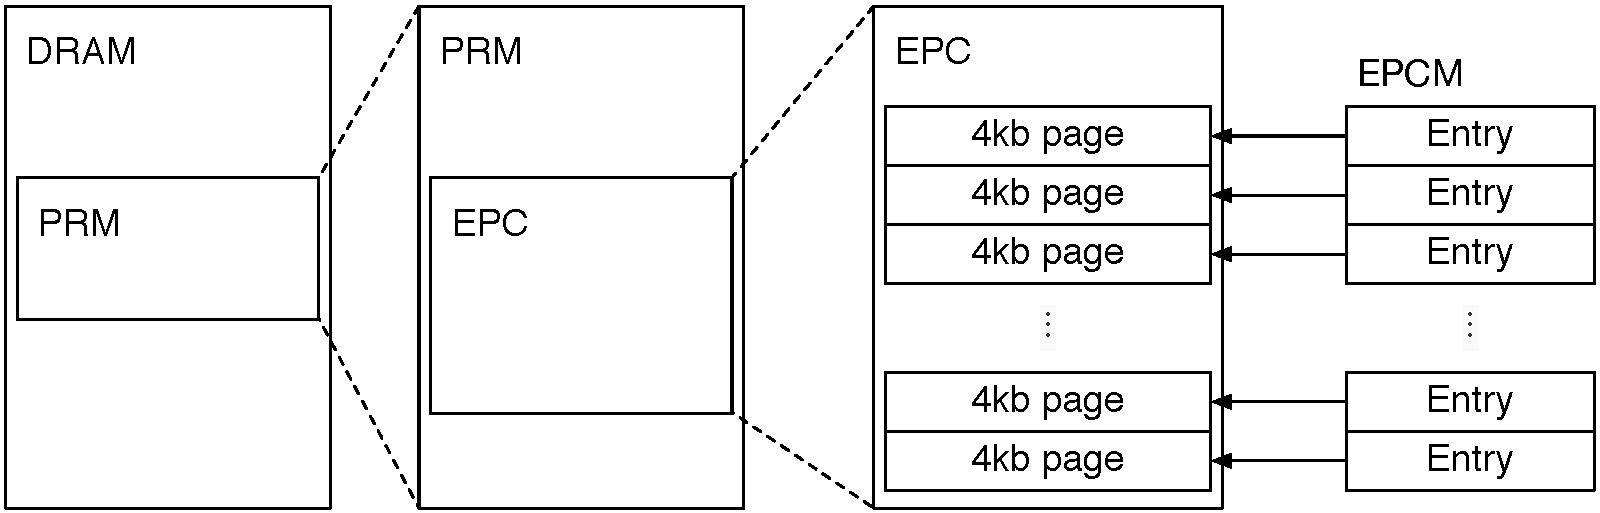
\includegraphics[width=87mm]{figures/sgx_epc.pdf}
  \caption{
    Enclave data is stored into the EPC, which is a subset of the PRM. The
    PRM is a contiguous range of DRAM that cannot be accessed by system
    software or peripherals.
  }
  \label{fig:sgx_epc}
\end{figure}

The SGX design supports having multiple enclaves on a system at the same time,
which is a necessity in multi-process environments. This is achieved by having
the EPC split into 4~KB pages that can be assigned to different enclaves. The
EPC uses the same page size as the architecture's address translation feature
(\S~\ref{sec:paging}). This is not a coincidence, as future sections will
reveal that the SGX implementation is tightly coupled with the address
translation implementation.

The EPC is managed by the same system software that manages the rest of the
computer's physical memory. The system software, which can be a hypervisor or
an OS kernel, uses SGX instructions to allocate unused pages to enclaves, and
to free previously allocated EPC pages. The system software is expected to
expose enclave creation and management services to application software.

Non-enclave software cannot directly access the EPC, as it is contained in the
PRM. This restriction plays a key role in SGX's enclave isolation guarantees,
but creates an obstacle when the system software needs to load the initial code
and data into a newly created enclave. The SGX design solves this problem by
having the instructions that allocate an EPC page to an enclave also initialize
the page. Most EPC pages are initialized by copying data from a non-PRM memory
page.


\HeadingLevelC{The Enclave Page Cache Map (EPCM)}
\label{sec:sgx_epcm}

% Enclave Page Cache Map (EPCM): SDM S 37.5.1, SDM S 38.19
% SECINFO.FLAGS: SDM S 38.11.1
% PAGE_TYPE Field Definition: SDM S 38.11.2

The SGX design expects the system software to allocate the EPC pages to
enclaves. However, as the system software is not trusted, SGX processors check
the correctness of the system software's allocation decisions, and refuse to
perform any action that would compromise SGX's security guarantees. For
example, if the system software attempts to allocate the same EPC page to two
enclaves, the SGX instruction used to perform the allocation will fail.

In order to perform its security checks, SGX records some information about the
system software's allocation decisions for each EPC page in the
\textit{Enclave Page Cache Map}~(EPCM). The EPCM is an array with one entry
per EPC page, so computing the address of a page's EPCM entry only requires a
bitwise shift operation and an addition.

The EPCM's contents is only used by SGX's security checks. Under normal
operation, the EPCM does not generate any software-visible behavior, and
enclave authors and system software developers can mostly ignore it.
Therefore, the SDM only describes the EPCM at a very high level, listing the
information contained within and noting that the EPCM is ``trusted memory''.
The SDM does not disclose the storage medium or memory layout used by the EPCM.

The EPCM uses the information in Table~\ref{fig:sgx_epcm_ownership_fields} to
track the ownership of each EPC page. We defer a full discussion of the EPCM to
a later section, because its contents is intimately coupled with all of SGX's
features, which will be described over the next few sections.

\begin{table}[hbt]
  \centering
  \begin{tabularx}{\columnwidth}{| l | r | X |}
  \hline
  \textbf{Field} & \textbf{Bits} & \textbf{Description}\\
  \hline
  VALID & 1 & 0 for un-allocated EPC pages \\
  \hline
  PT & 8 & page type \\
  \hline
  ENCLAVESECS &  & identifies the enclave owning the page \\
  \hline
  \end{tabularx}
  \caption{
    The fields in an EPCM entry that track the ownership of pages.
  }
  \label{fig:sgx_epcm_ownership_fields}
\end{table}

The SGX instructions that allocate an EPC page set the VALID bit of the
corresponding EPCM entry to 1, and refuse to operate on EPC pages whose VALID
bit is already set.

The instruction used to allocate an EPC page also determines the page's
intended usage, which is recorded in the \textit{page type} (PT) field of the
corresponding EPCM entry. The pages that store an enclave's code and data are
considered to have a \textit{regular} type (PT\_REG in the SDM). The pages
dedicated to the storage of SGX's supporting data structures are tagged with
special types. For example, the PT\_SECS type identifies pages that hold SGX
Enclave Control Structures, which will be described in the following section.
The other EPC page types will be described in future sections.

Last, a page's EPCM entry also identifies the enclave that owns the EPC page.
This information is used by the mechanisms that enforce SGX's isolation
guarantees to prevent an enclave from accessing another enclave's private
information. As the EPCM identifies a single owning enclave for each EPC page,
it is impossible for enclaves to communicate via shared memory using EPC pages.
Fortunately, enclaves can share untrusted non-EPC memory, as will be discussed
in \S~\ref{sec:sgx_paging}.


\HeadingLevelC{The SGX Enclave Control Structure (SECS)}
\label{sec:sgx_secs}

% Data Structures and Enclave Operation: SDM S 37.4
% SGX Enclave Control Structure (SECS): SDM S 38.7, S 38.7.1

SGX stores per-enclave metadata in a
\textit{SGX Enclave Control Structure}~(SECS) associated with each enclave.
Each SECS is stored in a dedicated EPC page with the page type PT\_SECS. These
pages are not intended to be mapped into any enclave's address space, and are
exclusively used by the CPU's SGX implementation.

% Constructing an Enclave: SDM S 39.1
% ECREATE: SDM S 39.1.1, S 41.3
% Implicit vs. Explicit accesses: SDM S 38.5.3
% Implicit accesses: SDM S 38.5.3.2

An enclave's identity is almost synonymous to its SECS. The first step in
bringing an enclave to life allocates an EPC page to serve as the enclave's
SECS, and the last step in destroying an enclave deallocates the page holding
its SECS. The EPCM entry field identifying the enclave that owns an EPC page
points to the enclave's SECS. The system software uses the virtual address of
an enclave's SECS to identify the enclave when invoking SGX instructions.

% Access Control Requirements: SDM S 38.3

All SGX instructions take virtual addresses as their inputs. Given that SGX
instructions use SECS addresses to identify enclaves, the system software must
create entries in its page tables pointing to the SECS of the enclaves it
manages. However, the system software cannot access any SECS page, as these
pages are stored in the PRM. SECS pages are not intended to be mapped inside
their enclaves' virtual address spaces, and SGX-enabled processors explicitly
prevent enclave code from accessing SECS pages.

% SGX Enclave Control Structure (SECS): SDM S 38.7, S 38.7.1

This seemingly arbitrary limitation is in place so that the SGX implementation
can store sensitive information in the SECS, and be able to assume that no
potentially malicious software will access that information. For example, the
SDM states that each enclave's measurement is stored in its SECS. If software
would be able to modify an enclave's measurement, SGX's software attestation
scheme would provide no security assurances.

The SECS is strongly coupled with many of SGX's features. Therefore, the pieces
of information that make up the SECS will be gradually introduced as the
different aspects of SGX are described.

\subsection{The Memory Layout of an SGX Enclave}
\label{sec:sgx_enclave_layout}

SGX was designed to minimize the effort required to convert application code to
take advantage of enclaves. History suggests this is a wise decision, as a
large factor in the continued dominance of the Intel architecture is its
ability to maintain backward compatibility. To this end, SGX enclaves were
designed to be conceptually similar to the leading software modularization
construct, dynamically loaded libraries, which are packaged as \texttt{.so}
files on Unix, and \texttt{.dll} files on Windows.

For simplicity, we describe the interaction between enclaves and non-enclave
software assuming that each enclave is used by exactly one application process,
which we shall refer to as the enclave's \textit{host process}. We do note,
however, that the SGX design does not explicitly prohibit multiple application
processes from sharing an enclave.


\subsubsection{The Enclave Linear Address Range (ELRANGE)}
\label{sec:sgx_elrange}

% SGX Enclave Control Structure (SECS): SDM S 38.7

Each enclave designates an area in its virtual address space, called the
\textit{enclave linear address range} (ELRANGE), which is used to map the code
and the sensitive data stored in the enclave's EPC pages. The virtual address
space outside ELRANGE is mapped to access non-EPC memory via the same virtual
addresses as the enclave's host process, as shown in
Figure~\ref{fig:sgx_elrange}.

\begin{figure}[hbt]
  \centering
  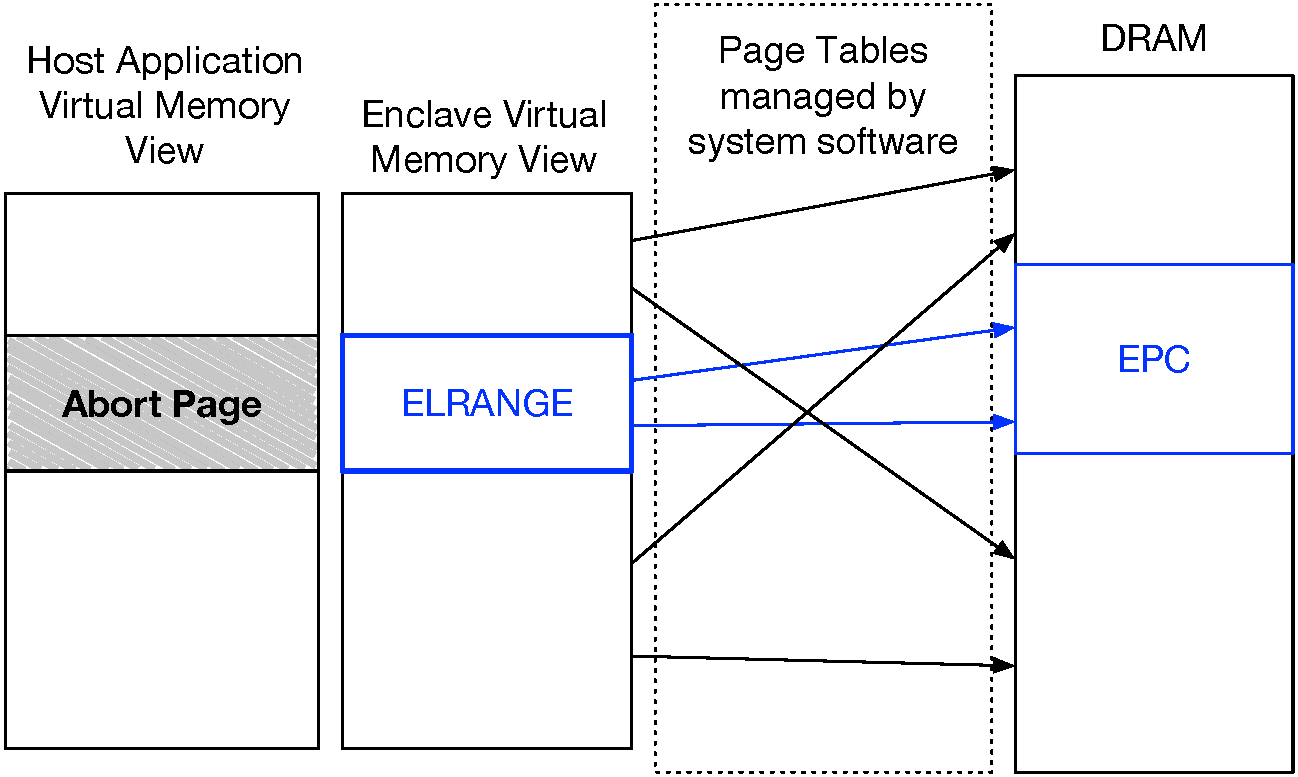
\includegraphics[width=85mm]{figures/sgx_elrange.pdf}
  \caption{
    An enclave's EPC pages are accessed using a dedicated region in the
    enclave's virtual address space, called ELRANGE. The rest of the virtual
    address space is used to access the memory of the host process. The memory
    mappings are established using the page tables managed by system software.
  }
  \label{fig:sgx_elrange}
\end{figure}

The SGX design guarantees that the enclave's memory accesses inside ELRANGE
obey the virtual memory abstraction~(\S~\ref{sec:paging_concepts}), while
memory accesses outside ELRANGE receive no guarantees. Therefore, enclaves must
store all their code and private data inside ELRANGE, and must consider the
memory outside ELRANGE to be an untrusted interface to the outside world.

The word ``linear'' in ELRANGE references the linear addresses produced by the
vestigial segmentation feature~(\S~\ref{sec:segments}) in the 64-bit Intel
architecture. For most purposes, ``linear'' can be treated as a synonym for
``virtual''.

ELRANGE is specified using a base (the BASEADDR field) and a size (the SIZE)
in the enclave's SECS~(\S~\ref{sec:sgx_secs}). ELRANGE must meet the same
constraints as a variable memory type range (\S~\ref{sec:cacheability_config})
and as the PRM range~(\S~\ref{sec:sgx_prm}), namely the size must be a power of
2, and the base must be aligned to the size. These restrictions are in place so
that the SGX implementation can inexpensively check whether an address belongs
to an enclave's ELRANGE, in either hardware~(\S~\ref{sec:cacheability_config})
or software.

When an enclave represents a dynamic library, it is natural to set ELRANGE to
the memory range reserved for the library by the loader. The ability to access
non-enclave memory from enclave code makes it easy to reuse existing library
code that expects to work with pointers to memory buffers managed by code in the
host process.


\subsubsection{SGX Enclave Attributes}
\label{sec:sgx_secs_attributes}

The execution environment of an enclave is heavily influenced by the value of
the ATTRIBUTES field in the enclave's SECS~(\S~\ref{sec:sgx_secs}). The rest of
this work will refer to the field's sub-fields, shown in
Table~\ref{fig:sgx_secs_attributes}, as \textit{enclave attributes}.

% ATTRIBUTES: SDM S 37.8.1

\begin{table}[hbt]
  \centering
  \begin{tabularx}{\columnwidth}{| l | r | X |}
  \hline
  \textbf{Field} & \textbf{Bits} & \textbf{Description} \\
  \hline
  DEBUG & 1 & Opts into enclave debugging features. \\
  \hline
  XFRM & 64 & The value of XCR0~(\S~\ref{sec:registers}) while this enclave's
              code is executed. \\
  \hline
  MODE64BIT & 1 & Set for 64-bit enclaves. \\
  \hline
  \end{tabularx}
  \caption{
    An enclave's attributes are the sub-fields in the ATTRIBUTES field of the
    enclave's SECS. This table shows a subset of the attributes defined in the
    SGX documentation.
  }
  \label{fig:sgx_secs_attributes}
\end{table}

The most important attribute, from a security perspective, is the DEBUG flag.
When this flag is set, it enables the use of SGX's debugging features for this
enclave. These debugging features include the ability to read and modify most
of the enclave's memory. Therefore, DEBUG should only be set in a development
environment, as it causes the enclave to lose all the SGX security guarantees.

SGX guarantees that enclave code will always run with the XCR0
register~(\S~\ref{sec:registers}) set to the value indicated by
\textit{extended features request mask}~(XFRM). Enclave authors are expected to
use XFRM to specify the set of architectural extensions enabled by the compiler
used to produce the enclave's code. Having XFRM be explicitly specified allows
Intel to design new architectural extensions that change the semantics of
existing instructions, such as Memory Protection Extensions (MPX), without
having to worry about the security implications on enclave code that was
developed without an awareness of the new features.

The MODE64BIT flag is set to true for enclaves that use the 64-bit Intel
architecture. From a security standpoint, this flag should not even exist, as
supporting a secondary architecture adds unnecessary complexity to the SGX
implementation, and increases the probability that security vulnerabilities
will creep in. In the interest of mental sanity, this work does not analyze the
behavior of SGX for enclaves whose MODE64BIT flag is cleared. However, a
security researcher who wishes to find vulnerabilities in SGX might study this
area.

Last, the INIT flag is always false when the enclave's SECS is created. The
flag is set to true at a certain point in the enclave lifecycle, which will be
summarized in \S~\ref{sec:sgx_enclave_lifecycle}.


\subsubsection{Address Translation for SGX Enclaves}
\label{sec:sgx_paging}

% Access Control Requirements: SDM S 38.3
% Interactions with VMX: SDM S 42.5, S 42.5.{1,2,3,4,5}

Under SGX, the operating system and hypervisor are still in full control of the
page tables and EPTs, and each enclave's code uses the same address translation
process and page tables~(\S~\ref{sec:paging}) as its host application. This
minimizes the amount of changes required to add SGX support to existing system
software. At the same time, having the page tables managed by untrusted system
software opens SGX up to the address translation attacks described in
\S~\ref{sec:address_translation_attacks}. As future sections will reveal, a
good amount of the complexity in SGX's design can be attributed to the need to
prevent these attacks.

SGX's active memory mapping attacks defense mechanisms revolve around ensuring
that each EPC page can only be mapped at a specific virtual
address~(\S~\ref{sec:segments}). When an EPC page is allocated, its intended
virtual address is recorded in the EPCM entry for the page, in the ADDRESS
field.

When an address translation (\S~\ref{sec:paging}) result is the physical
address of an EPC page, the CPU ensures\footnote{A mismatch triggers a general
protection fault (\#GP, \S~\ref{sec:faults}).} that the virtual address given
to the address translation process matches the expected virtual address
recorded in the page's EPCM entry.

SGX also protects against some passive memory mapping attacks and fault
injection attacks by ensuring that the access permissions of each EPC page
always match the enclave author's intentions. The access permissions for each
EPC page are specified when the page is allocated, and recorded in the
\textit{readable}~(R), \textit{writable}~(W), and \textit{executable}~(X)
fields in the page's EPCM entry, shown in
Table~\ref{fig:sgx_epcm_access_fields}.

\begin{table}[hbt]
  \centering
  \begin{tabularx}{\columnwidth}{| l | r | X |}
  \hline
  \textbf{Field} & \textbf{Bits} & \textbf{Description}\\
  \hline
  ADDRESS & 48 & the virtual address used to access this page\\
  \hline
  R & 1 & allow reads by enclave code\\
  \hline
  W & 1 & allow writes by enclave code\\
  \hline
  X & 1 & allow execution of code inside the page, inside enclave\\
  \hline
  \end{tabularx}
  \caption{
    The fields in an EPCM entry that indicate the enclave's intended virtual
    memory layout.
  }
  \label{fig:sgx_epcm_access_fields}
\end{table}

When an address translation (\S~\ref{sec:paging}) resolves into an EPC page,
the corresponding EPCM entry's fields override the access permission attributes
(\S~\ref{sec:page_table_attributes}) specified in the page tables. For example,
the W field in the EPCM entry overrides the writable (W) attribute, and the X
field overrides the disable execution (XD) attribute.

It follows that an enclave author must include memory layout information along
with the enclave, in such a way that the system software loading the enclave
will know the expected virtual memory address and access permissions for each
enclave page. In return, the SGX design guarantees to the enclave authors that
the system software, which manages the page tables and EPT, will not be able to
set up an enclave's virtual address space in a manner that is inconsistent with
the author's expectations.

The \texttt{.so} and \texttt{.dll} file formats, which are SGX's intended
enclave delivery vehicles, already have provisions for specifying the virtual
addresses that a software module was designed to use, as well as the desired
access permissions for each of the module's memory areas.

Last, a SGX-enabled CPU will ensure that the virtual memory inside
ELRANGE~(\S~\ref{sec:sgx_elrange}) is mapped to EPC pages. This prevents the
system software from carrying out an address translation attack where it maps
the enclave's entire virtual address space to DRAM pages outside the PRM, which
do not trigger any of the checks above, and can be directly accessed by the
system software.


\subsubsection{The Thread Control Structure (TCS)}
\label{sec:sgx_tcs}

% Thread Control Structure (TCS): SDM S 38.8, S 38.8.{1,2,3,4}

The SGX design fully embraces multi-core processors. It is possible for
multiple logical processors~(\S~\ref{sec:cpu_die}) to concurrently execute the
same enclave's code at the same time, via different threads.

The SGX implementation uses a \textit{Thread Control Structure}~(TCS) for each
logical processor that executes an enclave's code. It follows that an enclave's
author must provision at least as many TCS instances as the maximum number of
concurrent threads that the enclave is intended to support.

Each TCS is stored in a dedicated EPC page whose EPCM entry type is PT\_TCS.
The SDM describes the first few fields in the TCS. These fields are considered
to belong to the architectural part of the structure, and therefore are
guaranteed to have the same semantics on all the processors that support SGX.
The rest of the TCS is not documented.

% Access Control Requirements: SDM S 38.3
% EDBGRD, EDBGWR: SDM S 41.3

The contents of an EPC page that holds a TCS cannot be directly accessed, even
by the code of the enclave that owns the TCS. This restriction is similar to the
restriction on accessing EPC pages holding SECS instances. However, the
architectural fields in a TCS can be read by enclave debugging instructions.

The architectural fields in the TCS lay out the context
switches~(\S~\ref{sec:registers}) performed by a logical processor when it
transitions between executing non-enclave and enclave code.

For example, the OENTRY field specifies the value loaded in the instruction
pointer (RIP) when the TCS is used to start executing enclave code, so the
enclave author has strict control over the entry points available to enclave's
host application. Furthermore, the OFSBASGX and OFSBASGX fields specify the
base addresses loaded in the FS and GS segment
registers~(\S~\ref{sec:segments}), which typically point to Thread Local
Storage (TLS).


\subsubsection{The State Save Area (SSA)}
\label{sec:sgx_ssa}

% Interactions with the Processor Extended State and Miscellaneous State:
%     SDM S 42.7
% Requirements and Architecture Overview: SDM S 42.7.1

% State Save Area (SSA) Frame: SDM S 38.9

When the processor encounters a hardware exception~(\S~\ref{sec:faults}), such
as an interrupt~(\S~\ref{sec:interrupts}), while executing the code inside an
enclave, it performs a privilege level switch (\S~\ref{sec:faults}) and invokes
a hardware exception handler provided by the system software. Before executing
the exception handler, however, the processor needs a secure area to store the
enclave code's execution context~(\S~\ref{sec:registers}), so that the
information in the execution context is not revealed to the untrusted system
software.

% Relevant Fields in Various Data Structures: SDM S 42.7.2
% SECS.SSAFRAMESIZE: SDM S 42.7.2.2

In the SGX design, the area used to store an enclave thread's execution context
while a hardware exception is handled is called a \texttt{State Save
Area}~(SSA), illustrated in Figure~\ref{fig:sgx_enclave_layout}. Each TCS
references a contiguous sequence of SSAs. The \textit{offset of the SSA
array}~(OSSA) field specifies the location of the first SSA in the enclave's
virtual address space. The \textit{number of SSAs}~(NSSA) field indicates the
number of available SSAs.

\begin{figure}[hbt]
  \centering
  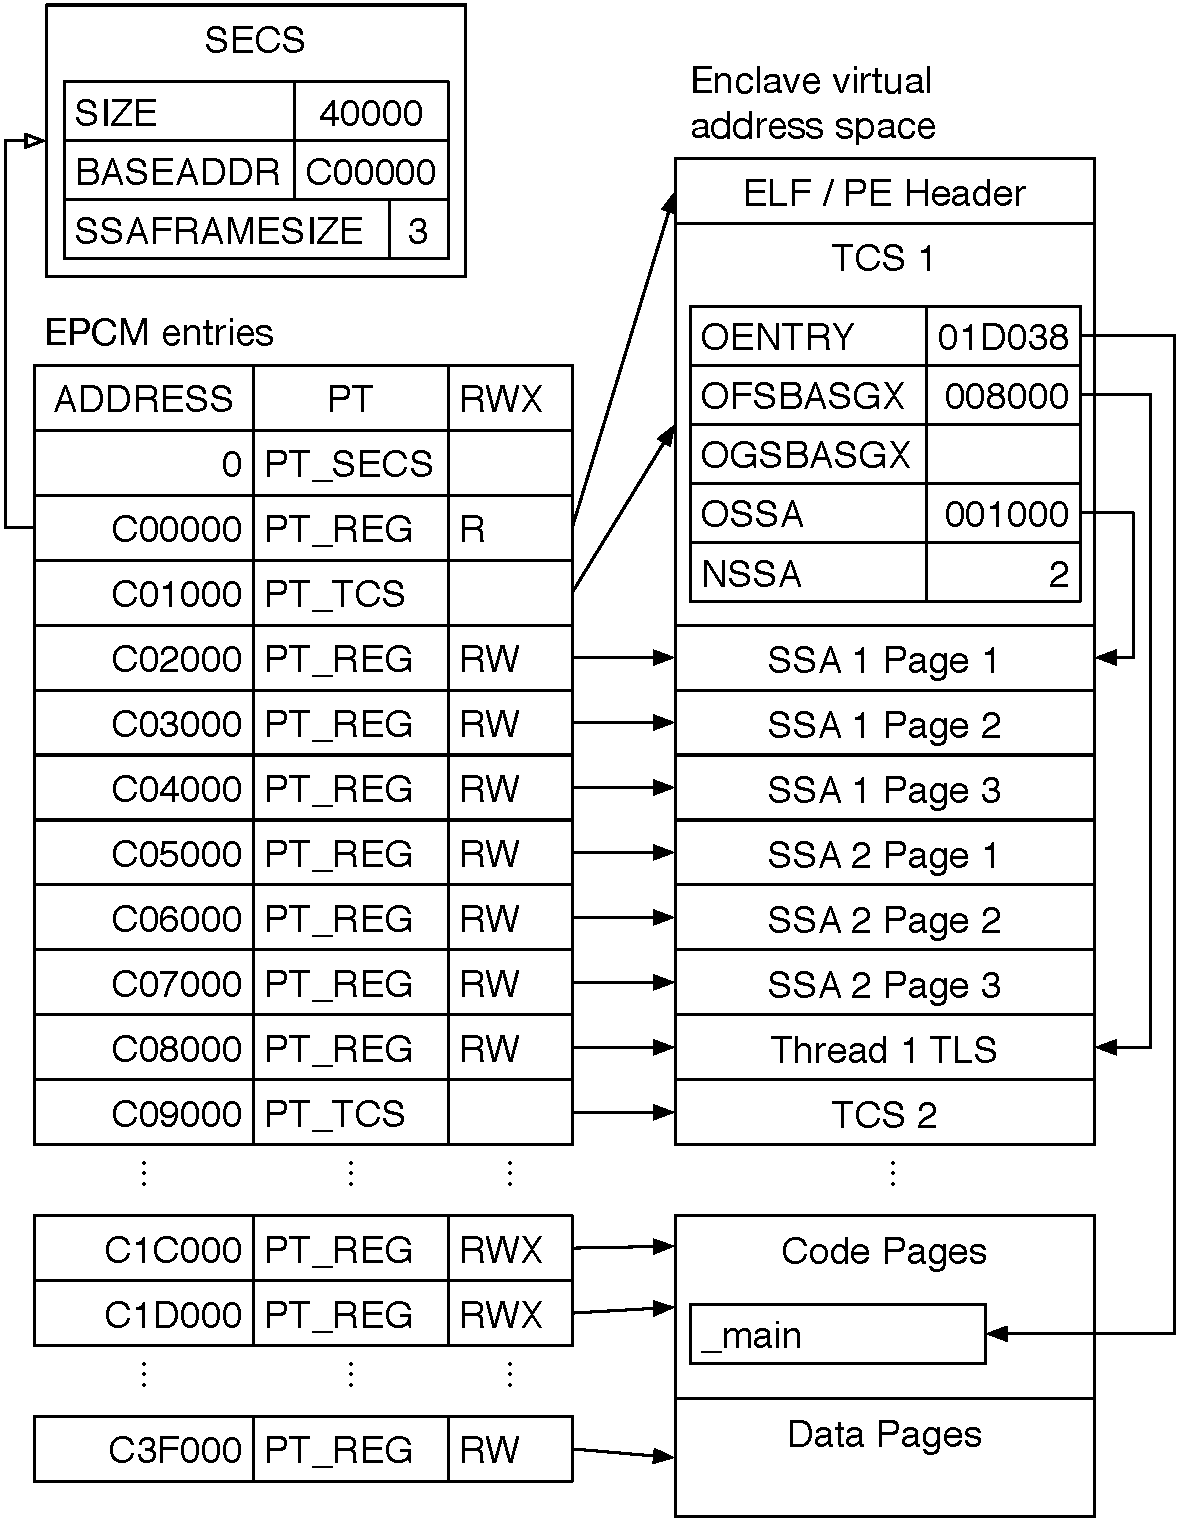
\includegraphics[width=85mm]{figures/sgx_enclave_layout.pdf}
  \caption{
    A possible layout of an enclave's virtual address space. Each enclave has a
    SECS, and one TCS per supported concurrent thread. Each TCS points to a
    sequence of SSAs, and specifies initial values for RIP and for the base
    addresses of FS and GS.
  }
  \label{fig:sgx_enclave_layout}
\end{figure}

Each SSA starts at the beginning of an EPC page, and uses up the number of EPC
pages that is specified in the SSAFRAMESIZE field of the enclave's SECS. These
alignment and size restrictions most likely simplify the SGX implementation by
reducing the number of special cases that it needs to handle.

% Relevant Fields in Various Data Structures: SDM S 42.7.2
% SECS.ATTRIBUTES.XFRM: SDM S 42.7.2.1

An enclave thread's execution context consists of the general-purpose registers
(GPRs) and the result of the XSAVE instruction~(\S~\ref{sec:registers}).
Therefore, the size of the execution context depends on the requested-feature
bitmap~(RFBM) used by to XSAVE. All the code in an enclave uses the same RFBM,
which is declared in the XFRM enclave
attribute~(\S~\ref{sec:sgx_secs_attributes}). The number of EPC pages reserved
for each SSA, specified in SSAFRAMESIZE,
must\footnote{\texttt{ECREATE}~(\S~\ref{sec:sgx_ecreate}) fails if SSAFRAMESIZE
is too small.} be large enough to fit the XSAVE output for the feature bitmap
specified by XFRM.

SSAs are stored in regular EPC pages, whose EPCM page type is PT\_REG.
Therefore, the SSA contents is accessible to enclave software. The SSA layout
is architectural, and is completely documented in the SDM. This opens up
possibilities for an enclave exception handler that is invoked by the host
application after a hardware exception occurs, and acts upon the information in
a SSA.

\subsection{The Life Cycle of an SGX Enclave}
\label{sec:sgx_enclave_lifecycle}

An enclave's life cycle is deeply intertwined with resource management,
specifically the allocation of EPC pages. Therefore, the instructions that
transition between different life cycle states can only be executed by the
system software. The system software is expected to expose the SGX instructions
described below as enclave loading and teardown services.

The following subsections describe the major steps in an enclave's lifecycle,
which is illustrated by Figure~\ref{fig:sgx_enclave_lifecycle}.

\begin{figure}[hbt]
  \centering
  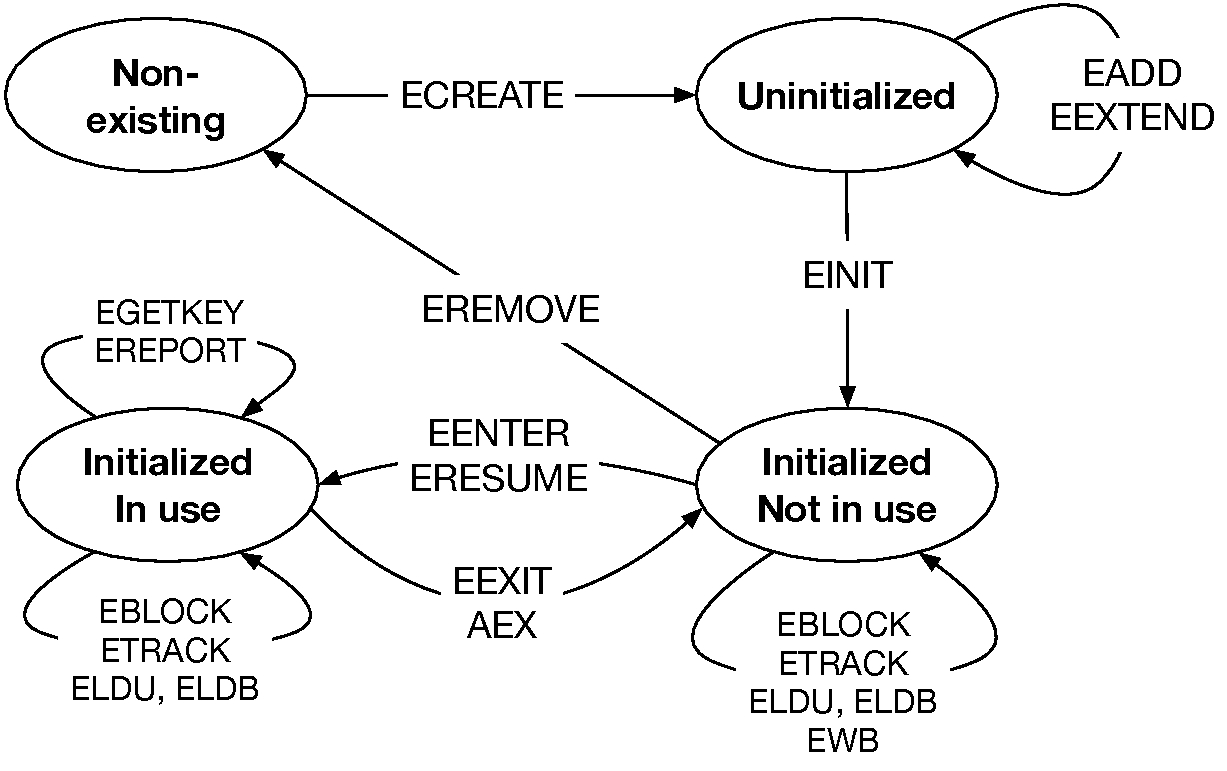
\includegraphics[width=85mm]{figures/sgx_enclave_lifecycle.pdf}
  \caption{
    The SGX enclave life cycle management instructions and state transition
    diagram
  }
  \label{fig:sgx_enclave_lifecycle}
\end{figure}


% Enclave Entry and Exiting : SDM S 39.2, S 39.2.1
% ECREATE, EADD, EREMOVE: SDM S 41.3

\subsubsection{Creation}
\label{sec:sgx_ecreate}

An enclave is born when the system software issues the \texttt{ECREATE}
instruction, which turns a free EPC page into the SECS~(\S~\ref{sec:sgx_secs})
for the new enclave.

\texttt{ECREATE} initializes the newly created SECS using the information in a
non-EPC page owned by the system software. This page specifies the values for
all the SECS fields defined in the SDM, such as BASEADDR and SIZE, using an
architectural layout that is guaranteed to be preserved by future
implementations.

While is very likely that the actual SECS layout used by initial SGX
implementations matches the architectural layout quite closely, future
implementations are free to deviate from this layout, as long as they maintain
the ability to initialize the SECS using the architectural layout.
Software cannot access an EPC page that holds a SECS, so it cannot become
dependent on an internal SECS layout. This is a stronger version of the
encapsulation used in the Virtual Machine Constrol
Structure~(VMCS,~\S~\ref{sec:vmx}).

\texttt{ECREATE} validates the information used to initialize the SECS, and
results in a page fault~(\#PF,~\S~\ref{sec:faults}) or general protection
fault~(\#GP,~\S~\ref{sec:faults}) if the information is not valid. For example,
if the SIZE field is not a power of two, \texttt{ECREATE} results in \#GP. This
validation, combined with the fact that the SECS is not accessible by software,
simplifies the implementation of the other SGX instructions, which can assume
that the information inside the SECS is valid.

Last, \texttt{ECREATE} initializes the enclave's INIT attribute (sub-field of
the ATTRIBUTES field in the enclave's SECS, \S~\ref{sec:sgx_secs_attributes})
to the false value. The enclave's code cannot be executed until the INIT
attribute is set to true, which happens in the initialization stage that will
be described in \S~\ref{sec:sgx_einit_overview}.


\subsubsection{Loading}
\label{sec:sgx_eadd}

\texttt{ECREATE} marks the newly created SECS as \textit{uninitialized}. While
an enclave's SECS is in this state, the system software can use \texttt{EADD}
instructions to load the initial code and data into the enclave. \texttt{EADD}
is used to create both TCS pages (\S~\ref{sec:sgx_tcs}) and regular pages.

% Page Information (PAGEINFO): SDM S 38.10
% Security Information (SECINFO): SDM S 38.11

\texttt{EADD} reads its input data from a \textit{Page Information}~(PAGEINFO)
structure, illustrated in Figure~\ref{fig:sgx_pageinfo}. The structure's
contents are only used to communicate information to the SGX implementation, so
it is entirely architectural and documented in the SDM.

\begin{figure}[hbt]
  \centering
  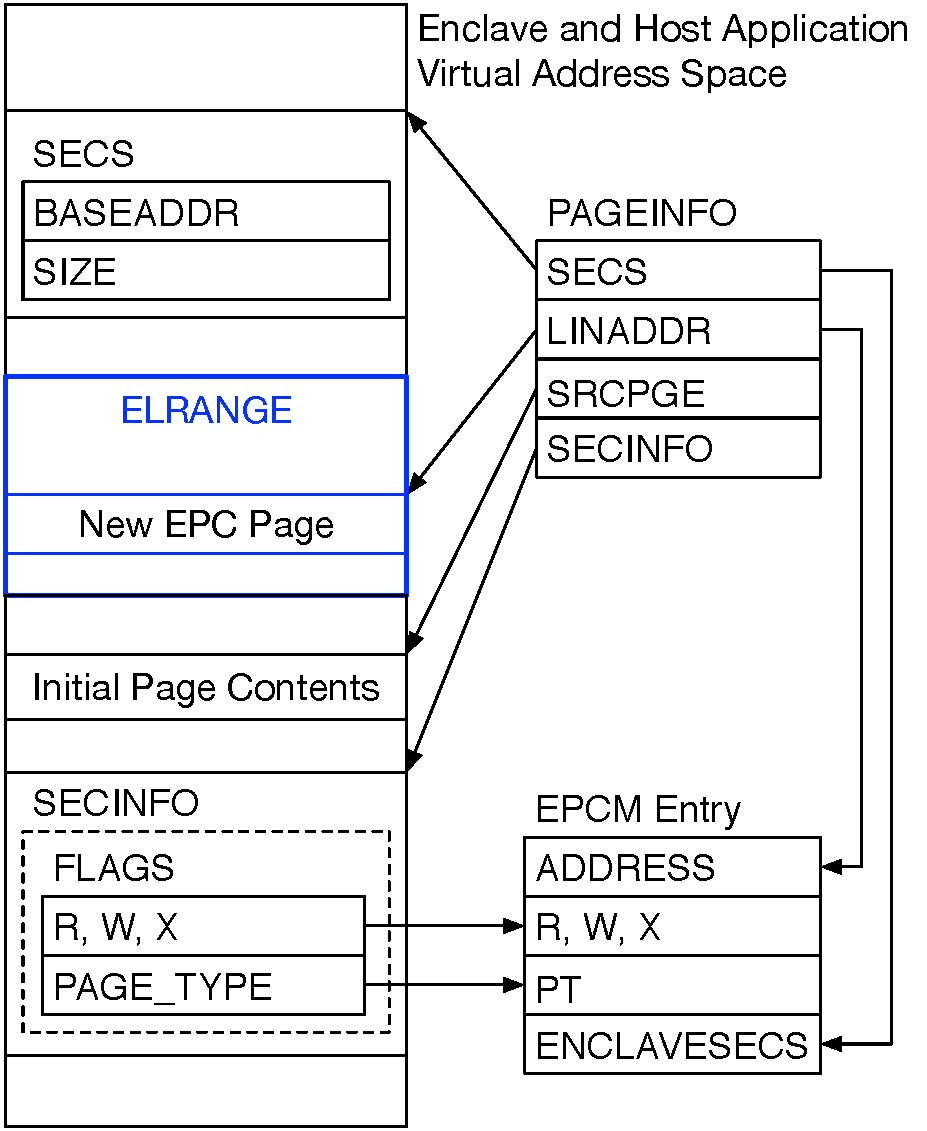
\includegraphics[width=65mm]{figures/sgx_pageinfo.pdf}
  \caption{
    The PAGEINFO structure supplies input data to SGX instructions such as
    \texttt{EADD}.
  }
  \label{fig:sgx_pageinfo}
\end{figure}

Currently, the PAGEINFO structure contains the virtual address of the EPC page
that will be allocated (LINADDR), the virtual address of the non-EPC page whose
contents will be copied into the newly allocated EPC page (SRCPGE), a virtual
address that resolves to the SECS of the enclave that will own the page (SECS),
and values for some of the fields of the EPCM entry associated with the newly
allocated EPC page (SECINFO).

The SECINFO field in the PAGEINFO structure is actually a virtual memory
address, and points to a \textit{Security Information}~(SECINFO) structure,
some of which is also illustrated in Figure~\ref{fig:sgx_pageinfo}. The SECINFO
structure contains the newly allocated EPC page's access permissions (R, W, X)
and its EPCM page type (PT\_REG or PT\_TCS). Like PAGEINFO, the SECINFO
structure is solely used to communicate data to the SGX implementation, so its
contents are also entirely architectural. However, most of the structure's
64 bytes are reserved for future use.

Both the PAGEINFO and the SECINFO structures are prepared by the system
software that invokes the \texttt{EADD} instruction, and therefore must be
contained in non-EPC pages. Both structures must be aligned to their sizes --
PAGEINFO is 32 bytes long, so each PAGEINFO instance must be 32-byte aligned,
while SECINFO has 64 bytes, and therefore each SECINFO instance must be
64-byte aligned. The alignment requirements likely simplify the SGX
implementation by reducing the number of special cases that must be handled.

\texttt{EADD} validates its inputs before modifying the newly allocated EPC
page or its EPCM entry. Most importantly, attempting to \texttt{EADD} a page to
an enclave whose SECS is in the initialized state will result in a \#GP.
Furthermore, attempting to \texttt{EADD} an EPC page that is already allocated
(the VALID field in its EPCM entry is 1) results in a \#PF. \texttt{EADD} also
ensures that the page's virtual address falls within the enclave's ELRANGE, and
that all the reserved fields in SECINFO are set to zero.

While loading an enclave, the system software will also use the
\texttt{EEXTEND} instruction, which updates the enclave's measurement used in
the software attestation process. Software attestation is discussed in
\S~\ref{sec:sgx_attestation}.


\subsubsection{Initialization}
\label{sec:sgx_einit_overview}

% EINIT Token Structure (EINITTOKEN): SDM S 38.14

After loading the initial code and data pages into the enclave, the system
software must use a \textit{Launch Enclave}~(LE) to obtain an EINIT Token
Structure, via an under-documented process that will be described in more
detail in \S~\ref{sec:sgx_launch_enclave}. The token is then provided to the
\texttt{EINIT} instruction, which marks the enclave's SECS as
\textit{initialized}.

The LE is a privileged enclave provided by Intel, and \textbf{is a prerequisite
for the use of enclaves authored by parties other than Intel}. The LE is an
SGX enclave, so it must be created, loaded and initialized using the processes
described in this section. However, the LE is cryptographically
signed~(\S~\ref{sec:integrity_crypto}) with a special Intel key that is
hard-coded into the SGX implementation, and that causes \texttt{EINIT} to
initialize the LE  without checking for a valid EINIT Token Structure.

When \texttt{EINIT} completes successfully, it sets the enclave's INIT
attribute to true. This opens the way for ring 3~(\S~\ref{sec:rings})
application software to execute the enclave's code, using the SGX instructions
described in \S~\ref{sec:sgx_threads}. On the other hand, once INIT is set to
true, \texttt{EADD} cannot be invoked on that enclave anymore, so the system
software must load all the pages that make up the enclave's initial state
before executing the \texttt{EINIT} instruction.


\subsubsection{Teardown}
\label{sec:sgx_eremove}

After the enclave has done the computation it was designed to perform, the
system software executes the \texttt{EREMOVE} instruction to deallocate the
EPC pages used by the enclave.

\texttt{EREMOVE} marks an EPC page as available by setting the VALID field of
the page's EPCM entry to 0 (zero). Before freeing up the page, \texttt{EREMOVE}
makes sure that there is no logical processor executing code inside the enclave
that owns the page to be removed.

An enclave is completely destroyed when the EPC page holding its SECS is freed.
\texttt{EREMOVE} refuses to deallocate a SECS page if it is referenced by any
other EPCM entry's ENCLAVESECS field, so an enclave's SECS page can only be
deallocated after all the enclave's pages have been deallocated.



